% Cálculo de Malliavin y aplicaciones en finanzas
% Compilar: latexmk -pdf main.tex   (o: pdflatex main && biber main && pdflatex main ×2)
\documentclass[11pt,a4paper]{report}
\usepackage[utf8]{inputenc}
\usepackage[T1]{fontenc}
\usepackage[spanish,es-noshorthands]{babel}
\usepackage{amsmath,amssymb,amsthm,mathtools,bm}
\usepackage{graphicx}
\usepackage[margin=2.5cm]{geometry}
\usepackage{hyperref}
\usepackage{xcolor}
\usepackage{listings}
\usepackage[backend=biber,style=alphabetic]{biblatex}
\addbibresource{referencias.bib}
\graphicspath{{../figures/}}

\newtheorem{teorema}{Teorema}[chapter]
\newtheorem{proposicion}[teorema]{Proposición}
\newtheorem{lema}[teorema]{Lema}
\newtheorem{corolario}[teorema]{Corolario}
\theoremstyle{definition}
\newtheorem{definicion}[teorema]{Definición}
\newtheorem{ejemplo}[teorema]{Ejemplo}
\theoremstyle{remark}
\newtheorem{observacion}[teorema]{Observación}

\newcommand{\R}{\mathbb{R}}
\newcommand{\E}{\mathbb{E}}
\newcommand{\Prob}{\mathbb{P}}
\newcommand{\Q}{\mathbb{Q}}
\newcommand{\F}{\mathcal{F}}
\newcommand{\Hil}{\mathcal{H}}
\newcommand{\D}{D}
\newcommand{\Dom}{\mathbb{D}^{1,2}}
\newcommand{\dive}{\delta}
\newcommand{\ind}{\mathbf{1}}
\newcommand{\ip}[2]{\langle #1, #2 \rangle}
\newcommand{\norm}[1]{\lVert #1 \rVert}
\newcommand{\dd}{\,\mathrm{d}}
\newcommand{\codigo}[1]{\texttt{#1}}


\title{Cálculo de Malliavin y aplicaciones en finanzas\\[0.3em]
\large Teoría, implementación numérica y visualización}
\author{}
\date{\today}

\begin{document}
\maketitle
\tableofcontents

\chapter{Introducción}

\paragraph{Relación con la guía teórica.} Este documento es el \emph{compañero
numérico} de la guía \emph{Cálculo de Malliavin: de los procesos estocásticos y la
integral de Itô al estado del arte} (\codigo{docs/pdf/Calculo\_de\_Malliavin\_corregido.pdf}),
que contiene las demostraciones completas. Aquí se adopta su notación y se cita su
numeración con la forma \guia{Teorema 8.9}. Cada resultado se acompaña de su
implementación y de una figura reproducible. La correspondencia capítulo a capítulo está en
\codigo{docs/mapa\_pdf.md}.

El cálculo de Malliavin es un cálculo diferencial en dimensión infinita sobre el
espacio de Wiener, introducido por P.~Malliavin \cite{malliavin1978} para dar una
prueba probabilística del teorema de hipoelipticidad de Hörmander. Su herramienta
central es una \emph{fórmula de integración por partes} que permite trasladar
derivadas desde una función hacia un \emph{peso} aleatorio:
\[
  \E\big[\varphi'(F)\,G\big] = \E\big[\varphi(F)\,H(F,G)\big].
\]
En finanzas esta identidad tiene tres usos principales, que recorre este documento:
\begin{enumerate}
  \item \textbf{Cobertura} (cap.~\ref{cap:clark-ocone}): la fórmula de
        Clark--Ocone identifica explícitamente la cartera replicante
        \cite{ocone1984,oconekaratzas1991}.
  \item \textbf{Sensibilidades} (cap.~\ref{cap:griegas}): las griegas se calculan
        por Monte Carlo sin derivar el pago, lo que es crucial para pagos
        discontinuos \cite{fournie1999,fournie2001,benhamou2003}.
  \item \textbf{Densidades y volatilidad implícita} (cap.~\ref{cap:densidades}), además de esperanzas condicionales y opciones bermudas \cite{bally2005}:
        existencia y estimación de densidades \cite{nualart2006} y desarrollos
        asintóticos de la volatilidad implícita \cite{alos2007,alosgarcialorite2021}.
\end{enumerate}

Cada resultado se acompaña de una implementación en la librería Python
\codigo{malliavin} (directorio \codigo{src/malliavin}) y de un script de
visualización en \codigo{examples/}; las figuras se incluyen desde
\codigo{figures/}. El capítulo~\ref{cap:implementacion} describe el mapa
fórmula~$\to$~función.

\paragraph{Notación.} $W=(W_t)_{t\in[0,T]}$ es un movimiento browniano estándar en
$(\Omega,\F,\Prob)$ con filtración natural $(\F_t)$; $\Hil=L^2([0,T])$ con producto
$\ip{h}{g}=\int_0^T h(t)g(t)\dd t$; $W(h)=\int_0^T h\dd W$ es la integral de Wiener.

\chapter{Espacio de Wiener y caos}

\section{Proceso isonormal}
La familia $\{W(h):h\in\Hil\}$ es un proceso gaussiano centrado con
$\E[W(h)W(g)]=\ip{h}{g}$. Denotamos por $He_n$ los polinomios de Hermite
probabilistas,
\[
  He_n(x) = (-1)^n e^{x^2/2}\frac{\dd^n}{\dd x^n}e^{-x^2/2},\qquad
  e^{tx-t^2/2}=\sum_{n\ge0}\frac{t^n}{n!}He_n(x).
\]

\section{Descomposición en caos}
\begin{teorema}[Wiener--Itô]
Toda $F\in L^2(\Omega,\F_T,\Prob)$ admite el desarrollo ortogonal
\[
  F = \sum_{n=0}^\infty I_n(f_n),\qquad \E[F^2]=\sum_{n\ge0} n!\,\norm{f_n}^2_{L^2([0,T]^n)},
\]
con $f_n$ simétricas y $I_n$ la integral múltiple de Itô.
\end{teorema}

Para funcionales que sólo dependen de $W_T$ basta con $h=\ind_{[0,T]}$:
$I_n(\ind_{[0,T]}^{\otimes n}) = T^{n/2} He_n(W_T/\sqrt T)$. Si $F=f(W_T)$ y $Z=W_T/\sqrt T$,
\[
  F=\sum_{n\ge0} a_n He_n(Z),\qquad a_n=\frac{\E[f(\sqrt T Z)He_n(Z)]}{n!},\qquad
  \operatorname{Var}(F)=\sum_{n\ge1} n!\,a_n^2.
\]

\begin{ejemplo}[Martingala exponencial]
$\exp(\sigma W_T-\tfrac12\sigma^2T)=\sum_n \frac{(\sigma\sqrt T)^n}{n!}He_n(Z)$:
el precio descontado de un activo log-normal vive en todos los caos con pesos
que decaen factorialmente.
\end{ejemplo}

\begin{figure}[h]
  \centering
  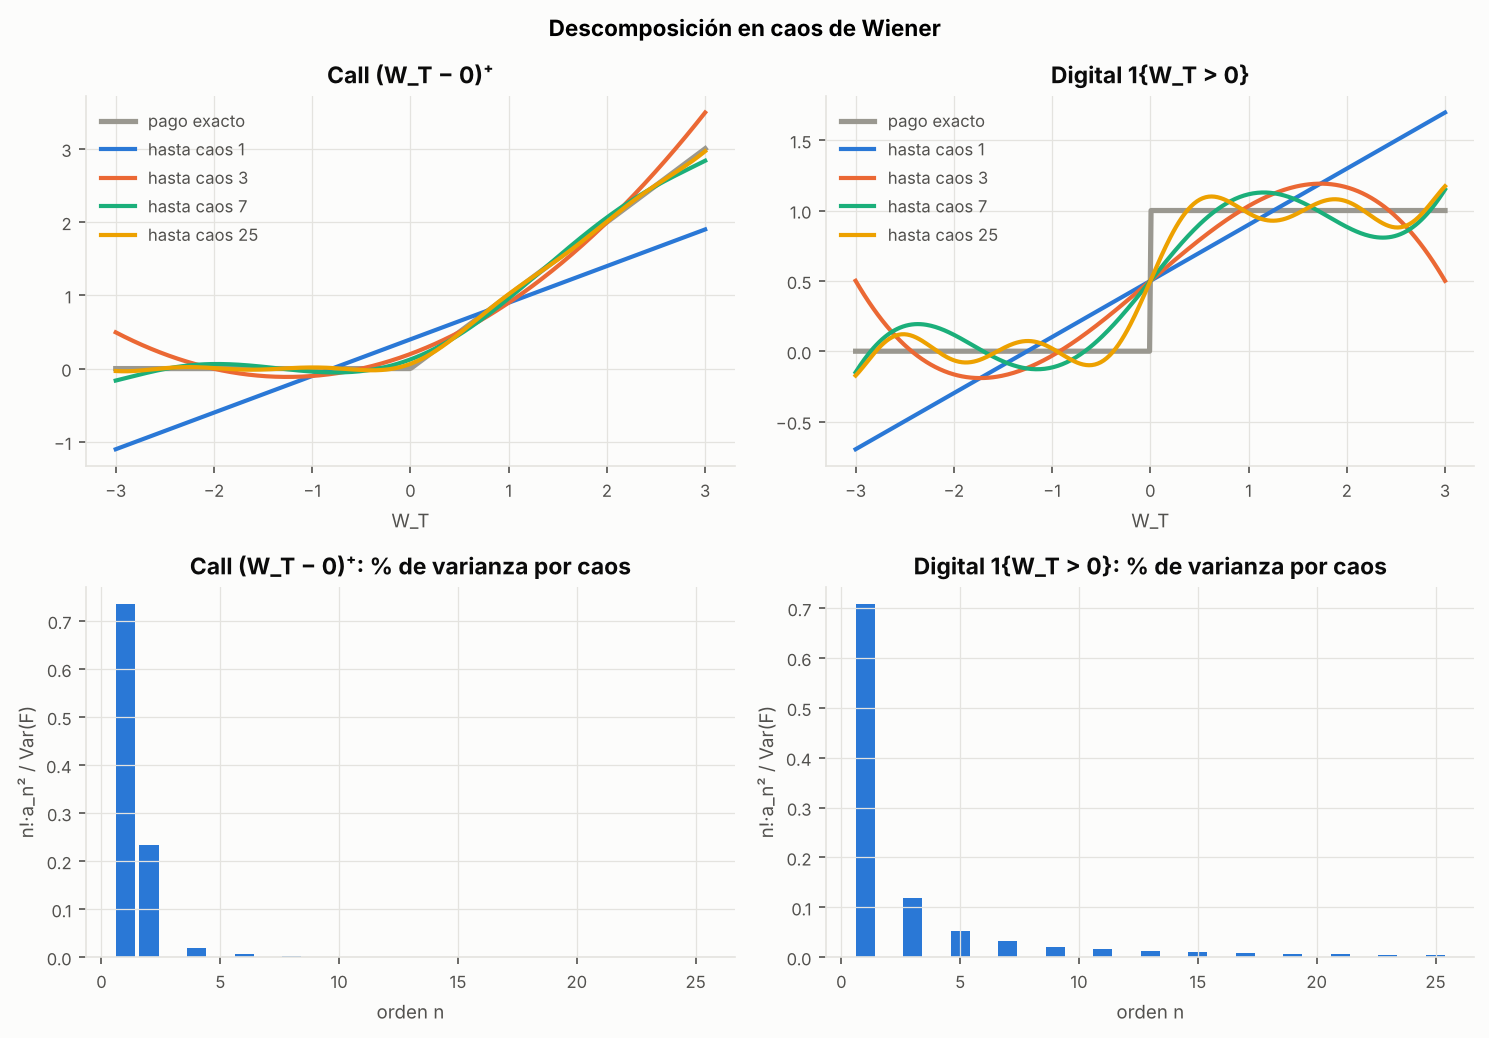
\includegraphics[width=\linewidth]{01_caos_de_wiener}
  \caption{Truncaciones del desarrollo en caos y energía por orden para una call
  y una digital (\codigo{examples/01\_caos\_de\_wiener.py}). La discontinuidad de la
  digital reparte la varianza en caos altos: decaimiento lento $\Rightarrow$ menor
  regularidad Malliavin.}
\end{figure}

\chapter{La derivada de Malliavin}

\section{Definición \guia{Definición 7.1}}
Sea $\mathcal S$ la clase de variables suaves $F=f(W(h_1),\dots,W(h_n))$ con
$f\in C_p^\infty(\R^n)$. Se define
\[
  \D_tF=\sum_{i=1}^n \partial_i f(W(h_1),\dots,W(h_n))\,h_i(t).
\]
$\D$ es cerrable de $L^2(\Omega)$ en $L^2(\Omega;\Hil)$; $\Dom$ es la clausura de
$\mathcal S$ para la norma $\norm{F}^2_{1,2}=\E[F^2]+\E\norm{\D F}^2_\Hil$.

\paragraph{Interpretación direccional.} Para $h\in\Hil$,
\[
  \ip{\D F}{h}=\lim_{\varepsilon\to0}\frac1\varepsilon\Big[F\big(\omega+\varepsilon\textstyle\int_0^\cdot h\big)-F(\omega)\Big],
\]
es decir, $\D F$ es el gradiente de $F$ en las direcciones de Cameron--Martin.

\section{Reglas de cálculo}
\begin{itemize}
  \item \textbf{Regla de la cadena:} $\D\,\varphi(F)=\varphi'(F)\D F$ para $\varphi\in C^1_b$
        (y para $\varphi$ Lipschitz con $\varphi'$ débil).
  \item \textbf{Caos:} $\D_t I_n(f_n)=n I_{n-1}(f_n(\cdot,t))$; por tanto
        $F\in\Dom \iff \sum_n n\,n!\norm{f_n}^2<\infty$.
  \item \textbf{Adaptación:} si $F$ es $\F_s$-medible, $\D_tF=0$ para $t>s$.
\end{itemize}

\section{Ejemplos}
\begin{center}
\begin{tabular}{ll}
  $F$ & $\D_tF$, \ $t\in[0,T]$\\\hline
  $W_T^p$ & $pW_T^{p-1}$\\
  $\int_0^T W_s\dd s$ & $T-t$\\
  $\max_{s\le T}W_s$ & $\ind_{[0,\tau^*]}(t)$, \ $\tau^*=\arg\max$ \guia{Prop.~7.16}\\
  $S_T=S_0e^{(r-\sigma^2/2)T+\sigma W_T}$ & $\sigma S_T$\\
  $\int_0^T S_u\dd u$ & $\sigma\int_t^T S_u\dd u$\\
\end{tabular}
\end{center}

\section{Versión discreta}
Si $F=\phi(\Delta W_0,\dots,\Delta W_{n-1})$ sobre una malla $t_k=kT/n$, entonces
$\D_tF=\partial\phi/\partial(\Delta W_k)$ para $t\in[t_k,t_{k+1})$. Esta es la
aproximación que implementa \codigo{derivative.discrete\_malliavin\_derivative}.

\begin{figure}[h]
  \centering
  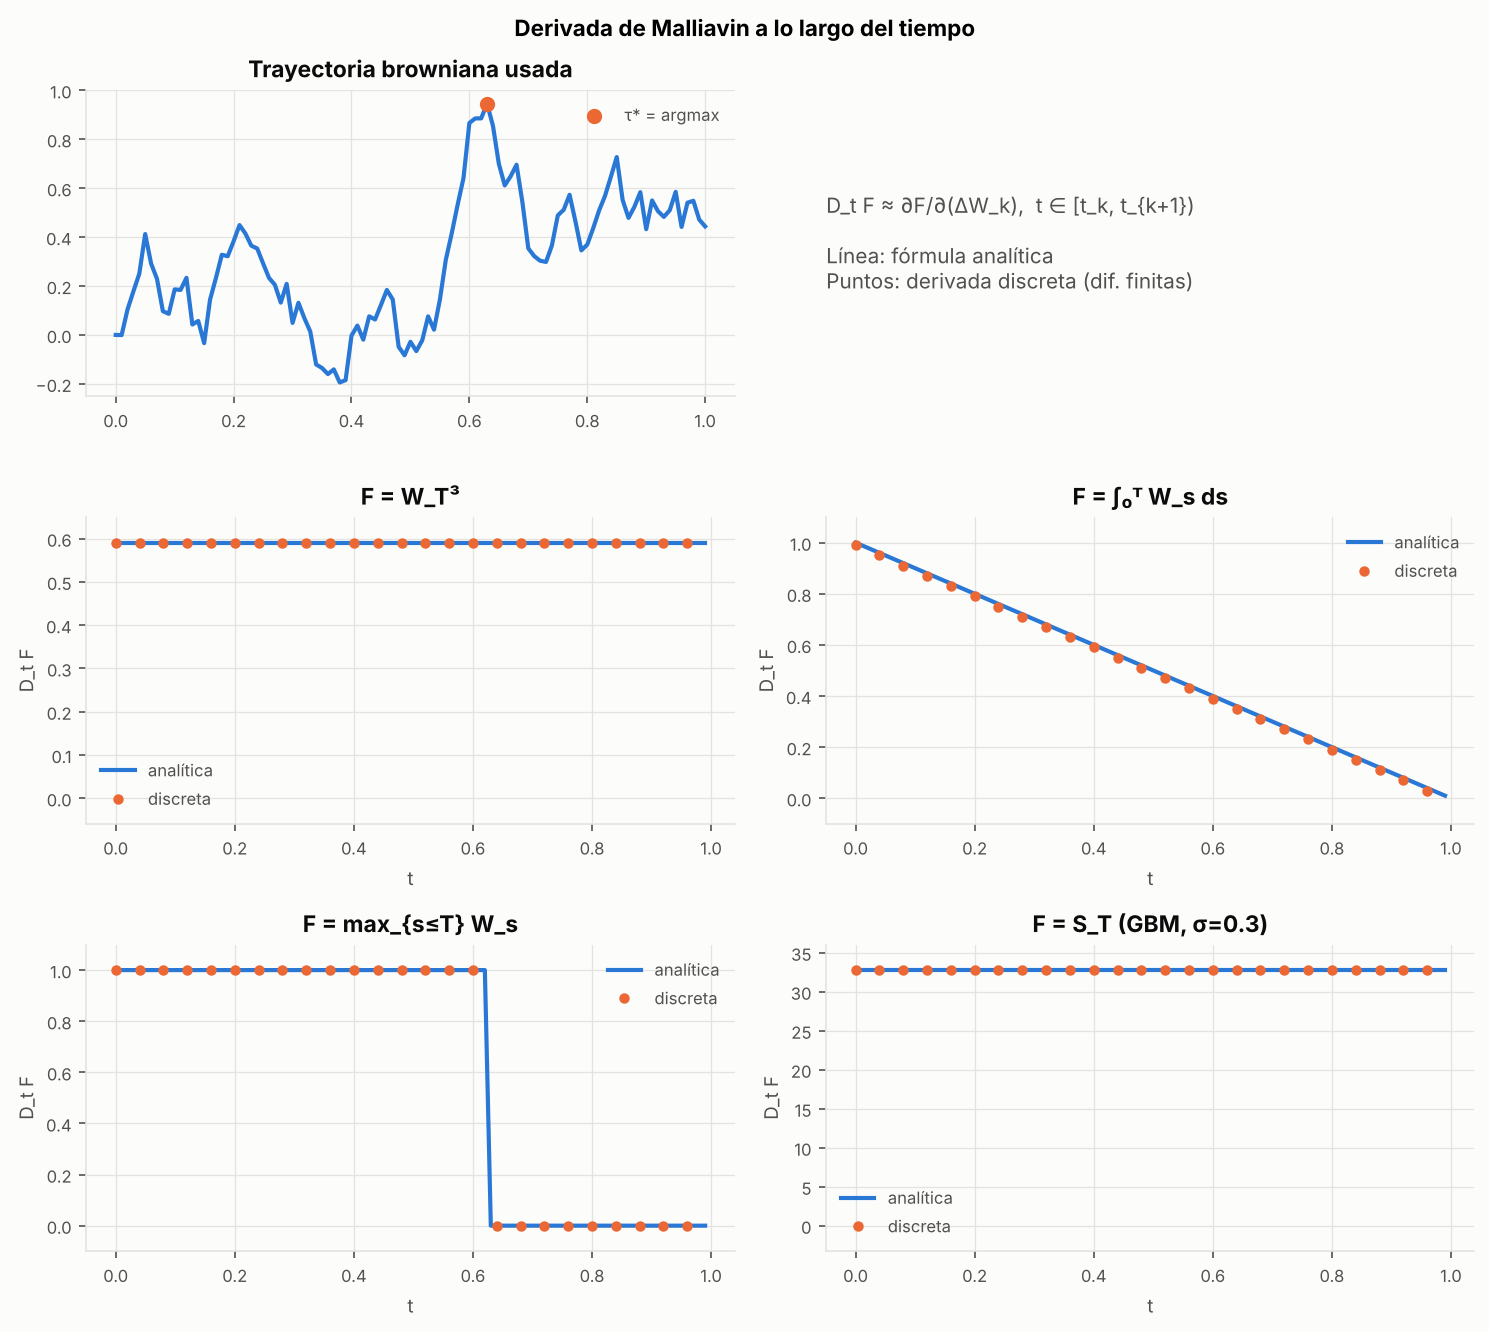
\includegraphics[width=0.9\linewidth]{02_derivada_malliavin}
  \caption{Derivada discreta frente a la analítica (\codigo{examples/02\_derivada\_malliavin.py}).}
\end{figure}

\chapter{Divergencia e integral de Skorokhod}

\begin{definicion}
El operador divergencia $\dive$ es el adjunto de $\D$: $u\in L^2(\Omega;\Hil)$ está en
$\operatorname{Dom}\dive$ si $|\E\ip{\D F}{u}|\le c\norm{F}_{L^2}$ para toda $F\in\mathcal S$, y entonces
\begin{equation}\label{eq:ibp}
  \E\big[\ip{\D F}{u}\big]=\E\big[F\,\dive(u)\big].
\end{equation}
\end{definicion}

\begin{proposicion}
\begin{enumerate}
  \item Si $h$ es determinista, $\dive(h)=W(h)$.
  \item Si $u$ es adaptado y de cuadrado integrable, $\dive(u)=\int_0^Tu_t\dd W_t$ (Itô).
  \item Si $G\in\Dom$ y $Gu\in\operatorname{Dom}\dive$: $\dive(Gu)=G\dive(u)-\ip{\D G}{u}$.
\end{enumerate}
\end{proposicion}

Por (2), $\dive$ extiende la integral de Itô a integrandos anticipativos: es la
integral de Skorokhod \cite{skorokhod1975}.

\begin{ejemplo}
Con $u_t=W_T$ (no adaptado), por (3): $\dive(W_T)=W_TW_T-\ip{\ind}{\ind}=W_T^2-T$.
Tomando $F=W_T^2$ en \eqref{eq:ibp}: $\E[2W_T\cdot W_T\cdot T]=2T^2=\E[W_T^2(W_T^2-T)]$.
\end{ejemplo}

\paragraph{Lema clave para finanzas.} Si $\ip{\D F}{u}\neq0$ c.s., aplicando
\eqref{eq:ibp} a $\varphi(F)$ con integrando $u/\ip{\D F}{u}$:
\begin{equation}\label{eq:peso}
  \E[\varphi'(F)G]=\E\Big[\varphi(F)\,\dive\Big(\frac{G\,u}{\ip{\D F}{u}}\Big)\Big].
\end{equation}

\begin{figure}[h]
  \centering
  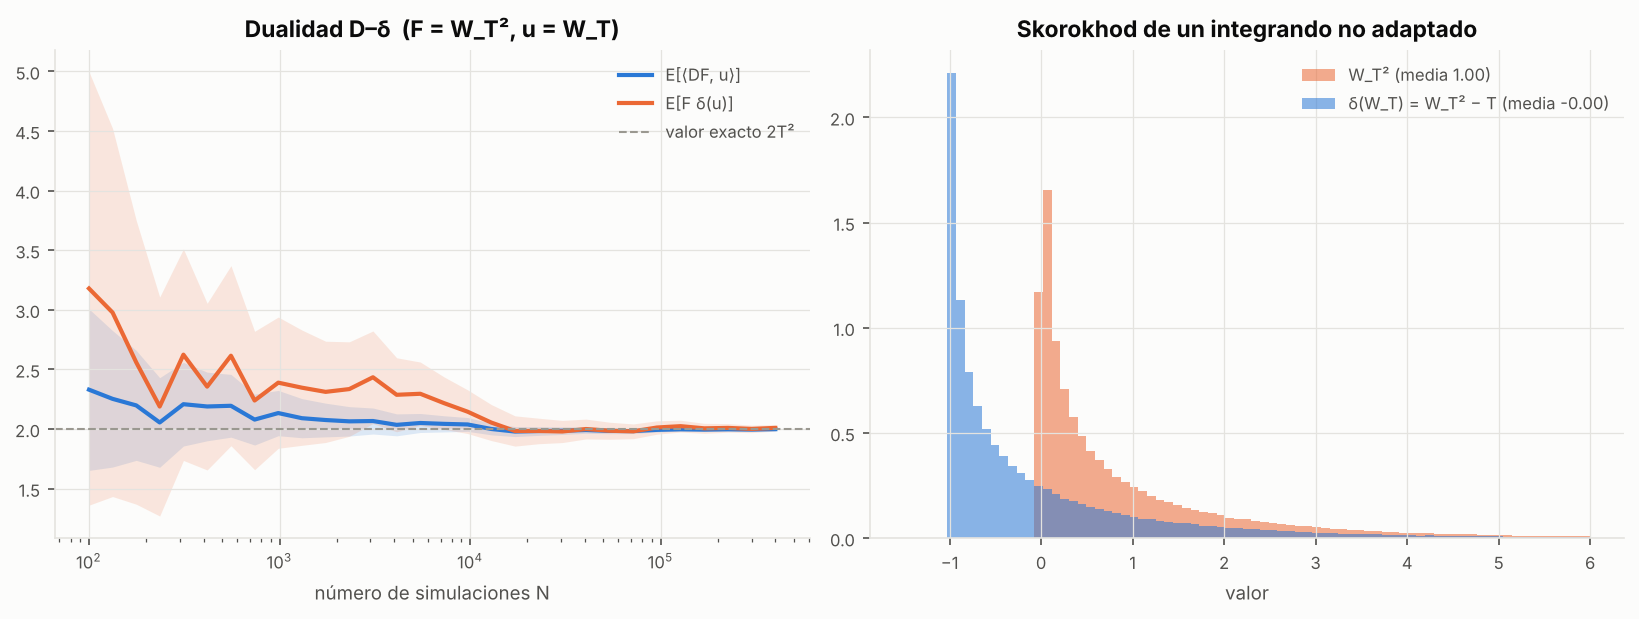
\includegraphics[width=0.95\linewidth]{03_integracion_por_partes}
  \caption{Verificación Monte Carlo de la dualidad y comparación
  $\dive(W_T)$ vs.\ $W_T^2$ (\codigo{examples/03\_integracion\_por\_partes.py}).}
\end{figure}

\chapter{Fórmula de Clark--Ocone y cobertura}\label{cap:clark-ocone}

\begin{teorema}[Clark--Ocone, \guia{Teorema 8.9}]
Si $F\in\Dom$ es $\F_T$-medible,
\[
  F=\E[F]+\int_0^T\E[\D_tF\mid\F_t]\dd W_t.
\]
\end{teorema}

\begin{ejemplo}
$F=W_T^3$: $\D_tF=3W_T^2$ y $\E[3W_T^2\mid\F_t]=3(W_t^2+T-t)$.
\end{ejemplo}

\section{Cobertura en Black--Scholes}
Bajo $\Q$, $\dd S_t=rS_t\dd t+\sigma S_t\dd W_t$ y $\tilde S_t=e^{-rt}S_t$ cumple
$\dd\tilde S_t=\sigma\tilde S_t\dd W_t$. Para el pago descontado
$F=e^{-rT}\Phi(S_T)$, Clark--Ocone da
\[
  F=\E_\Q[F]+\int_0^T\phi_t\dd W_t=\E_\Q[F]+\int_0^T\Delta_t\dd\tilde S_t,\qquad
  \Delta_t=\frac{\phi_t}{\sigma\tilde S_t}.
\]
Para la call, $\D_tF=e^{-rT}\ind_{\{S_T>K\}}\sigma S_T$ y
$\E[\D_tF\mid\F_t]=\sigma\tilde S_t\,N(d_1(t))$: se recupera la delta de
Black--Scholes, $\Delta_t=N(d_1(t))$ \guia{Ejemplo 13.2}. Para la digital
\guia{Ejemplo 13.3}, $\Delta_t=e^{-r(T-t)}\varphi(d_2)/(\sigma S_t\sqrt{T-t})$ para $t<T$
(\codigo{clark\_ocone.integrand\_digital}). La ventaja del enfoque es que se generaliza a
pagos dependientes de la trayectoria y a modelos sin EDP explícita
\cite{oconekaratzas1991,dinunno2009}.

\begin{figure}[h]
  \centering
  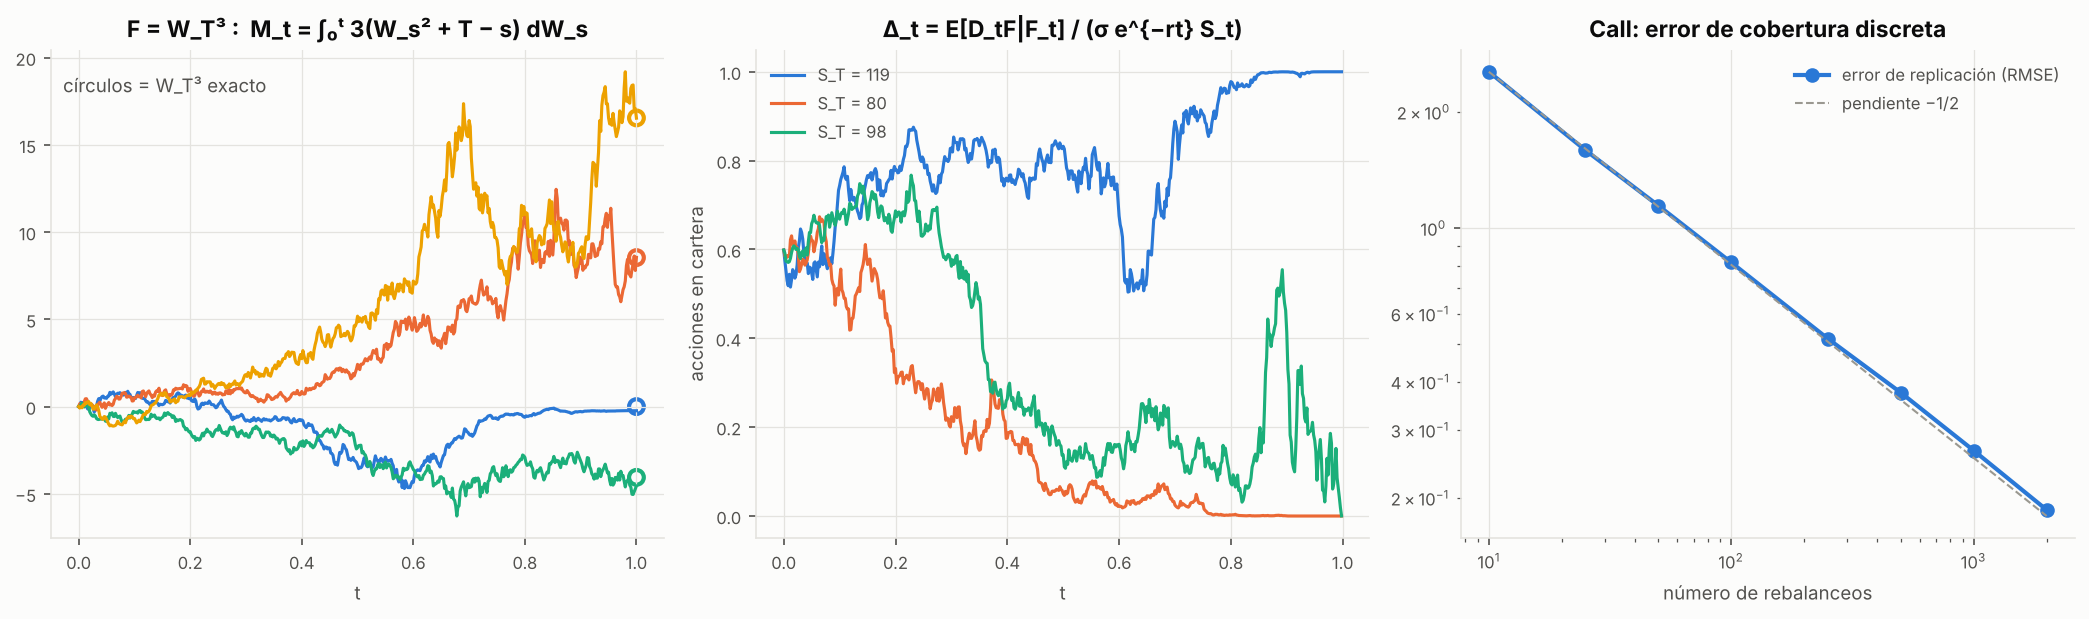
\includegraphics[width=\linewidth]{04_clark_ocone_cobertura}
  \caption{Reconstrucción de $W_T^3$, deltas de cobertura y error de replicación
  discreto $\propto n^{-1/2}$ (\codigo{examples/04\_clark\_ocone\_cobertura.py}).}
\end{figure}

\chapter{Griegas por pesos de Malliavin}\label{cap:griegas}

Sea $V(\theta)=\E[e^{-rT}\Phi(S_T^\theta)]$. Las diferencias finitas tienen sesgo
$O(h^2)$ y varianza $O(h^{-2})$ (o $O(h^{-3})$ para la gamma) si $\Phi$ es
discontinua; el método \emph{pathwise} exige $\Phi$ diferenciable. Aplicando
\eqref{eq:peso} \cite{fournie1999}:
\[
  \partial_\theta V=\E\big[e^{-rT}\Phi(S_T)\,\pi_\theta\big],
\]
con pesos que no dependen de $\Phi$. En el modelo de Black--Scholes:
\begin{align*}
  \pi_\Delta&=\frac{W_T}{S_0\sigma T}, &
  \pi_{\mathcal V}&=\frac{W_T^2}{\sigma T}-W_T-\frac1\sigma,\\
  \pi_\Gamma&=\frac{\pi_{\mathcal V}}{S_0^2\sigma T}, &
  \pi_\rho&=\frac{W_T}{\sigma}-T.
\end{align*}

\paragraph{Derivación de $\pi_\Delta$.} $\partial_{S_0}V=e^{-rT}\E[\Phi'(S_T)S_T/S_0]$ y
$\ip{\D S_T}{\ind}=\sigma S_TT$. Con $u=\ind$ y $G=S_T/S_0$ en \eqref{eq:peso}:
$\dive\big(\tfrac{1}{S_0\sigma T}\big)=\tfrac{W_T}{S_0\sigma T}$.

\section{Opción asiática}
Sea $A=\frac1T\int_0^TS_t\dd t$. Con $u_t=S_t$:
$\ip{\D A}{u}=\tfrac{\sigma}{T}\int_0^TS_s\int_s^TS_t\dd t\dd s=\tfrac{\sigma T}{2}A^2$, y
\[
  \Delta=\frac{e^{-rT}}{S_0}\E\Big[\Phi(A)\Big(\frac{2(S_T-S_0)}{\sigma^2TA}-\frac{2r}{\sigma^2}+1\Big)\Big].
\]

\begin{observacion}
Para pagos suaves (call) el estimador de Malliavin puede tener \emph{más} varianza
que el pathwise; las técnicas de localización y pesos óptimos
\cite{fournie2001,benhamou2003} combinan lo mejor de ambos.
\end{observacion}

\begin{figure}[h]
  \centering
  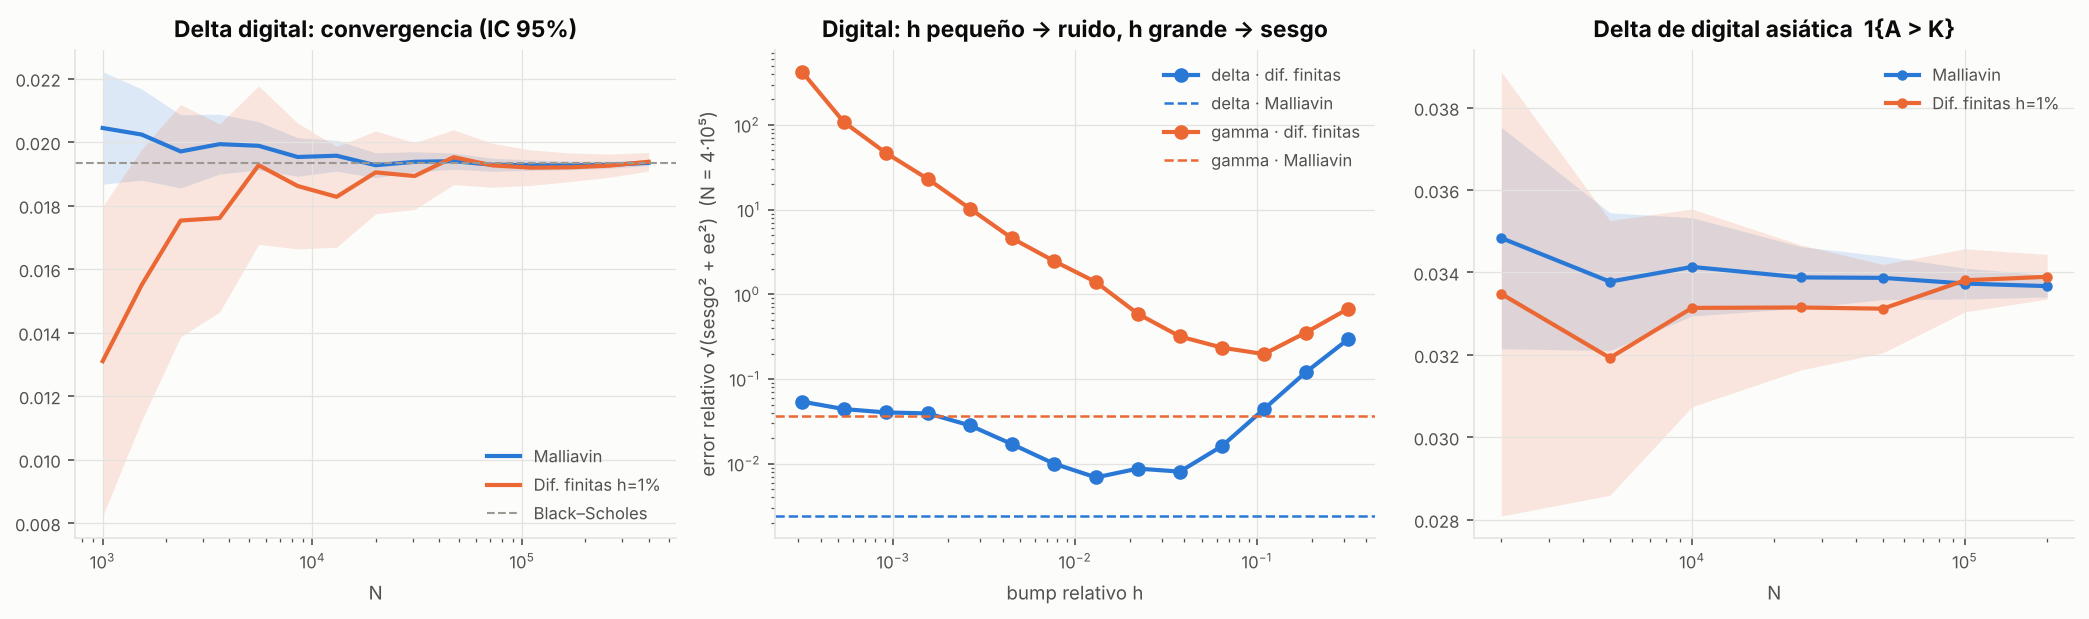
\includegraphics[width=\linewidth]{05_griegas_malliavin}
  \caption{Delta digital, compromiso sesgo--varianza en $h$, y delta de una digital
  asiática (\codigo{examples/05\_griegas\_malliavin.py}).}
\end{figure}

\chapter{Densidades}\label{cap:densidades}

\begin{proposicion}[{\guia{Teorema 10.1}, \cite[Prop.~2.1.1]{nualart2006}}]
Si $F\in\Dom$ y $\D F/\norm{\D F}_\Hil^2\in\operatorname{Dom}\dive$, $F$ tiene densidad
continua
\[
  p_F(x)=\E\Big[\ind_{\{F>x\}}\,\dive\Big(\frac{\D F}{\norm{\D F}^2_\Hil}\Big)\Big].
\]
\end{proposicion}

Para $F=S_T$: $\D F=\sigma S_T\ind_{[0,T]}$, $\norm{\D F}^2=\sigma^2S_T^2T$ y
\[
  \dive\Big(\frac{1}{\sigma TS_T}\Big)=\frac1{S_T}\Big(\frac{W_T}{\sigma T}+1\Big).
\]
El estimador resultante es insesgado en cada punto y no requiere ancho de banda.
Las mismas ideas sustentan la expansión de la volatilidad implícita en
\cite{alos2007,alosgarcialorite2021}.

\begin{figure}[h]
  \centering
  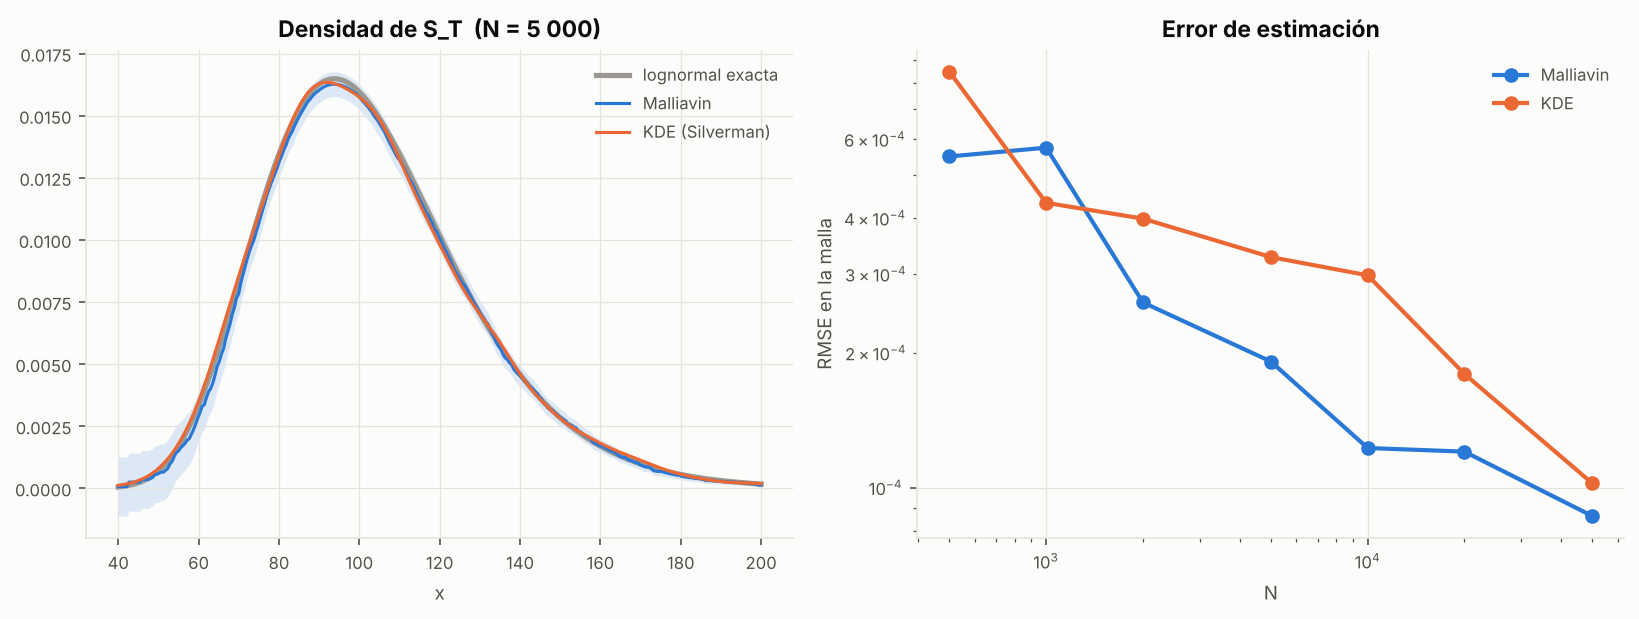
\includegraphics[width=0.95\linewidth]{06_densidad_malliavin}
  \caption{Densidad de $S_T$: Malliavin vs.\ KDE (\codigo{examples/06\_densidad\_malliavin.py}).}
\end{figure}

\chapter{Implementación}\label{cap:implementacion}

\begin{center}
\begin{tabular}{lll}
  Concepto & Fórmula & Función\\\hline
  Caos & $a_n=\E[fHe_n]/n!$ & \codigo{chaos.chaos\_coefficients}\\
  Derivada discreta & $\partial\phi/\partial\Delta W_k$ & \codigo{derivative.discrete\_malliavin\_derivative}\\
  Skorokhod producto & $G\dive(h)-\ip{\D G}{h}$ & \codigo{skorokhod.skorokhod\_product}\\
  Clark--Ocone & $\E[\D_tF\mid\F_t]$ & \codigo{clark\_ocone.integrand\_*}\\
  Griegas & $\E[\Phi\,\pi_\theta]$ & \codigo{greeks.greeks\_malliavin}\\
  Asiática & $\pi_\Delta^{A}$ & \codigo{greeks.asian\_delta\_malliavin}\\
  Densidad & $\E[\ind_{F>x}\dive(\cdot)]$ & \codigo{density.gbm\_terminal\_density}\\
\end{tabular}
\end{center}

Las identidades de los capítulos anteriores se verifican automáticamente en
\codigo{tests/test\_malliavin.py} (\codigo{pytest}).


\printbibliography[heading=bibintoc,title={Bibliografía}]
\end{document}
